\documentclass[11pt]{beamer}
\usetheme{JuanLesPins}
\usepackage[utf8]{inputenc}
\usepackage[english]{babel}
\usepackage{amsmath}
\usepackage{amsfonts}
\usepackage{amssymb}
\usepackage{graphicx}
\author{Camila Celeste RIBA PEREYRA}
\title{An introduction to Beamer}
%\setbeamercovered{transparent} 
%\setbeamertemplate{navigation symbols}{} 
\logo{isterre.png}
\institute{ISTerre - USMB} 
\date{\today}
\subject{Magnetotellurics} 
\begin{document}


\section{Introduction}
\begin{frame}[plain]
	\titlepage
\end{frame}

\begin{frame}
\tableofcontents
\end{frame}


\section{Basic facts about ducks}
\subsection{Blocs}
\begin{frame}{Blocs 1/2}
	\begin{center}
		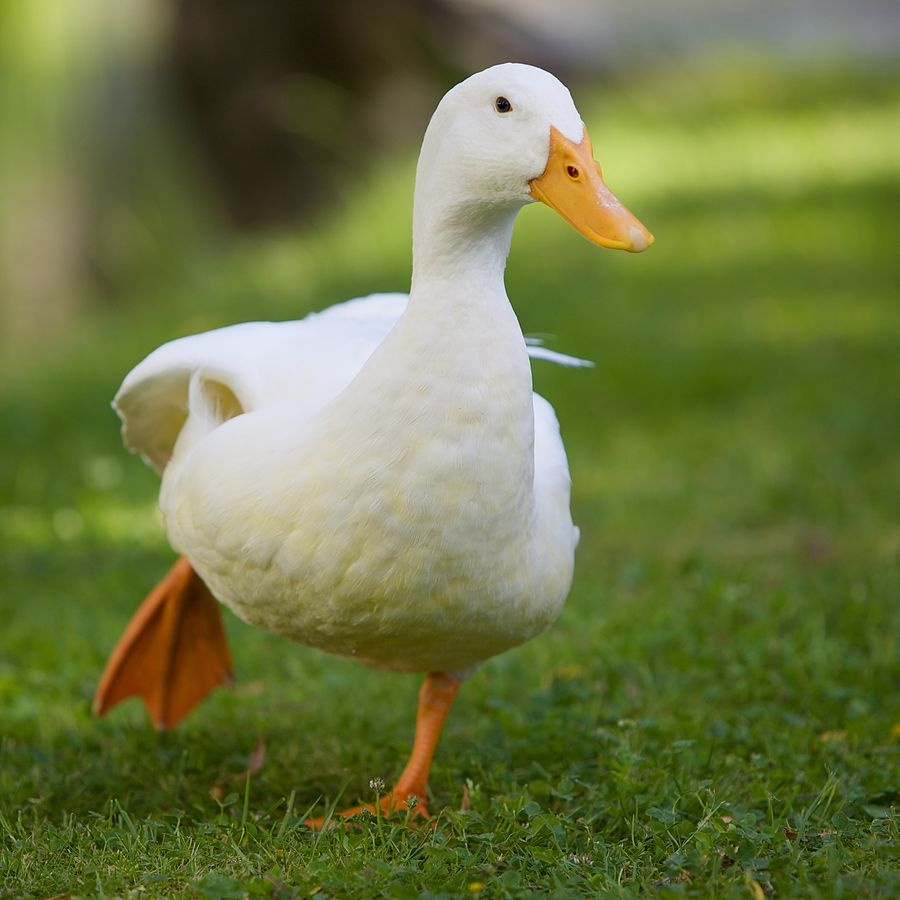
\includegraphics[width = .5\textwidth]{runningduck.jpg}
	\end{center}
	\begin{block} {A standard block}
		\begin{itemize}
			\item Ducks are famous for their hunting skills
			\item Number two
		\end{itemize}
	\end{block}
\end{frame}

\begin{frame}{Blocs 2/2}
	\begin{center}
		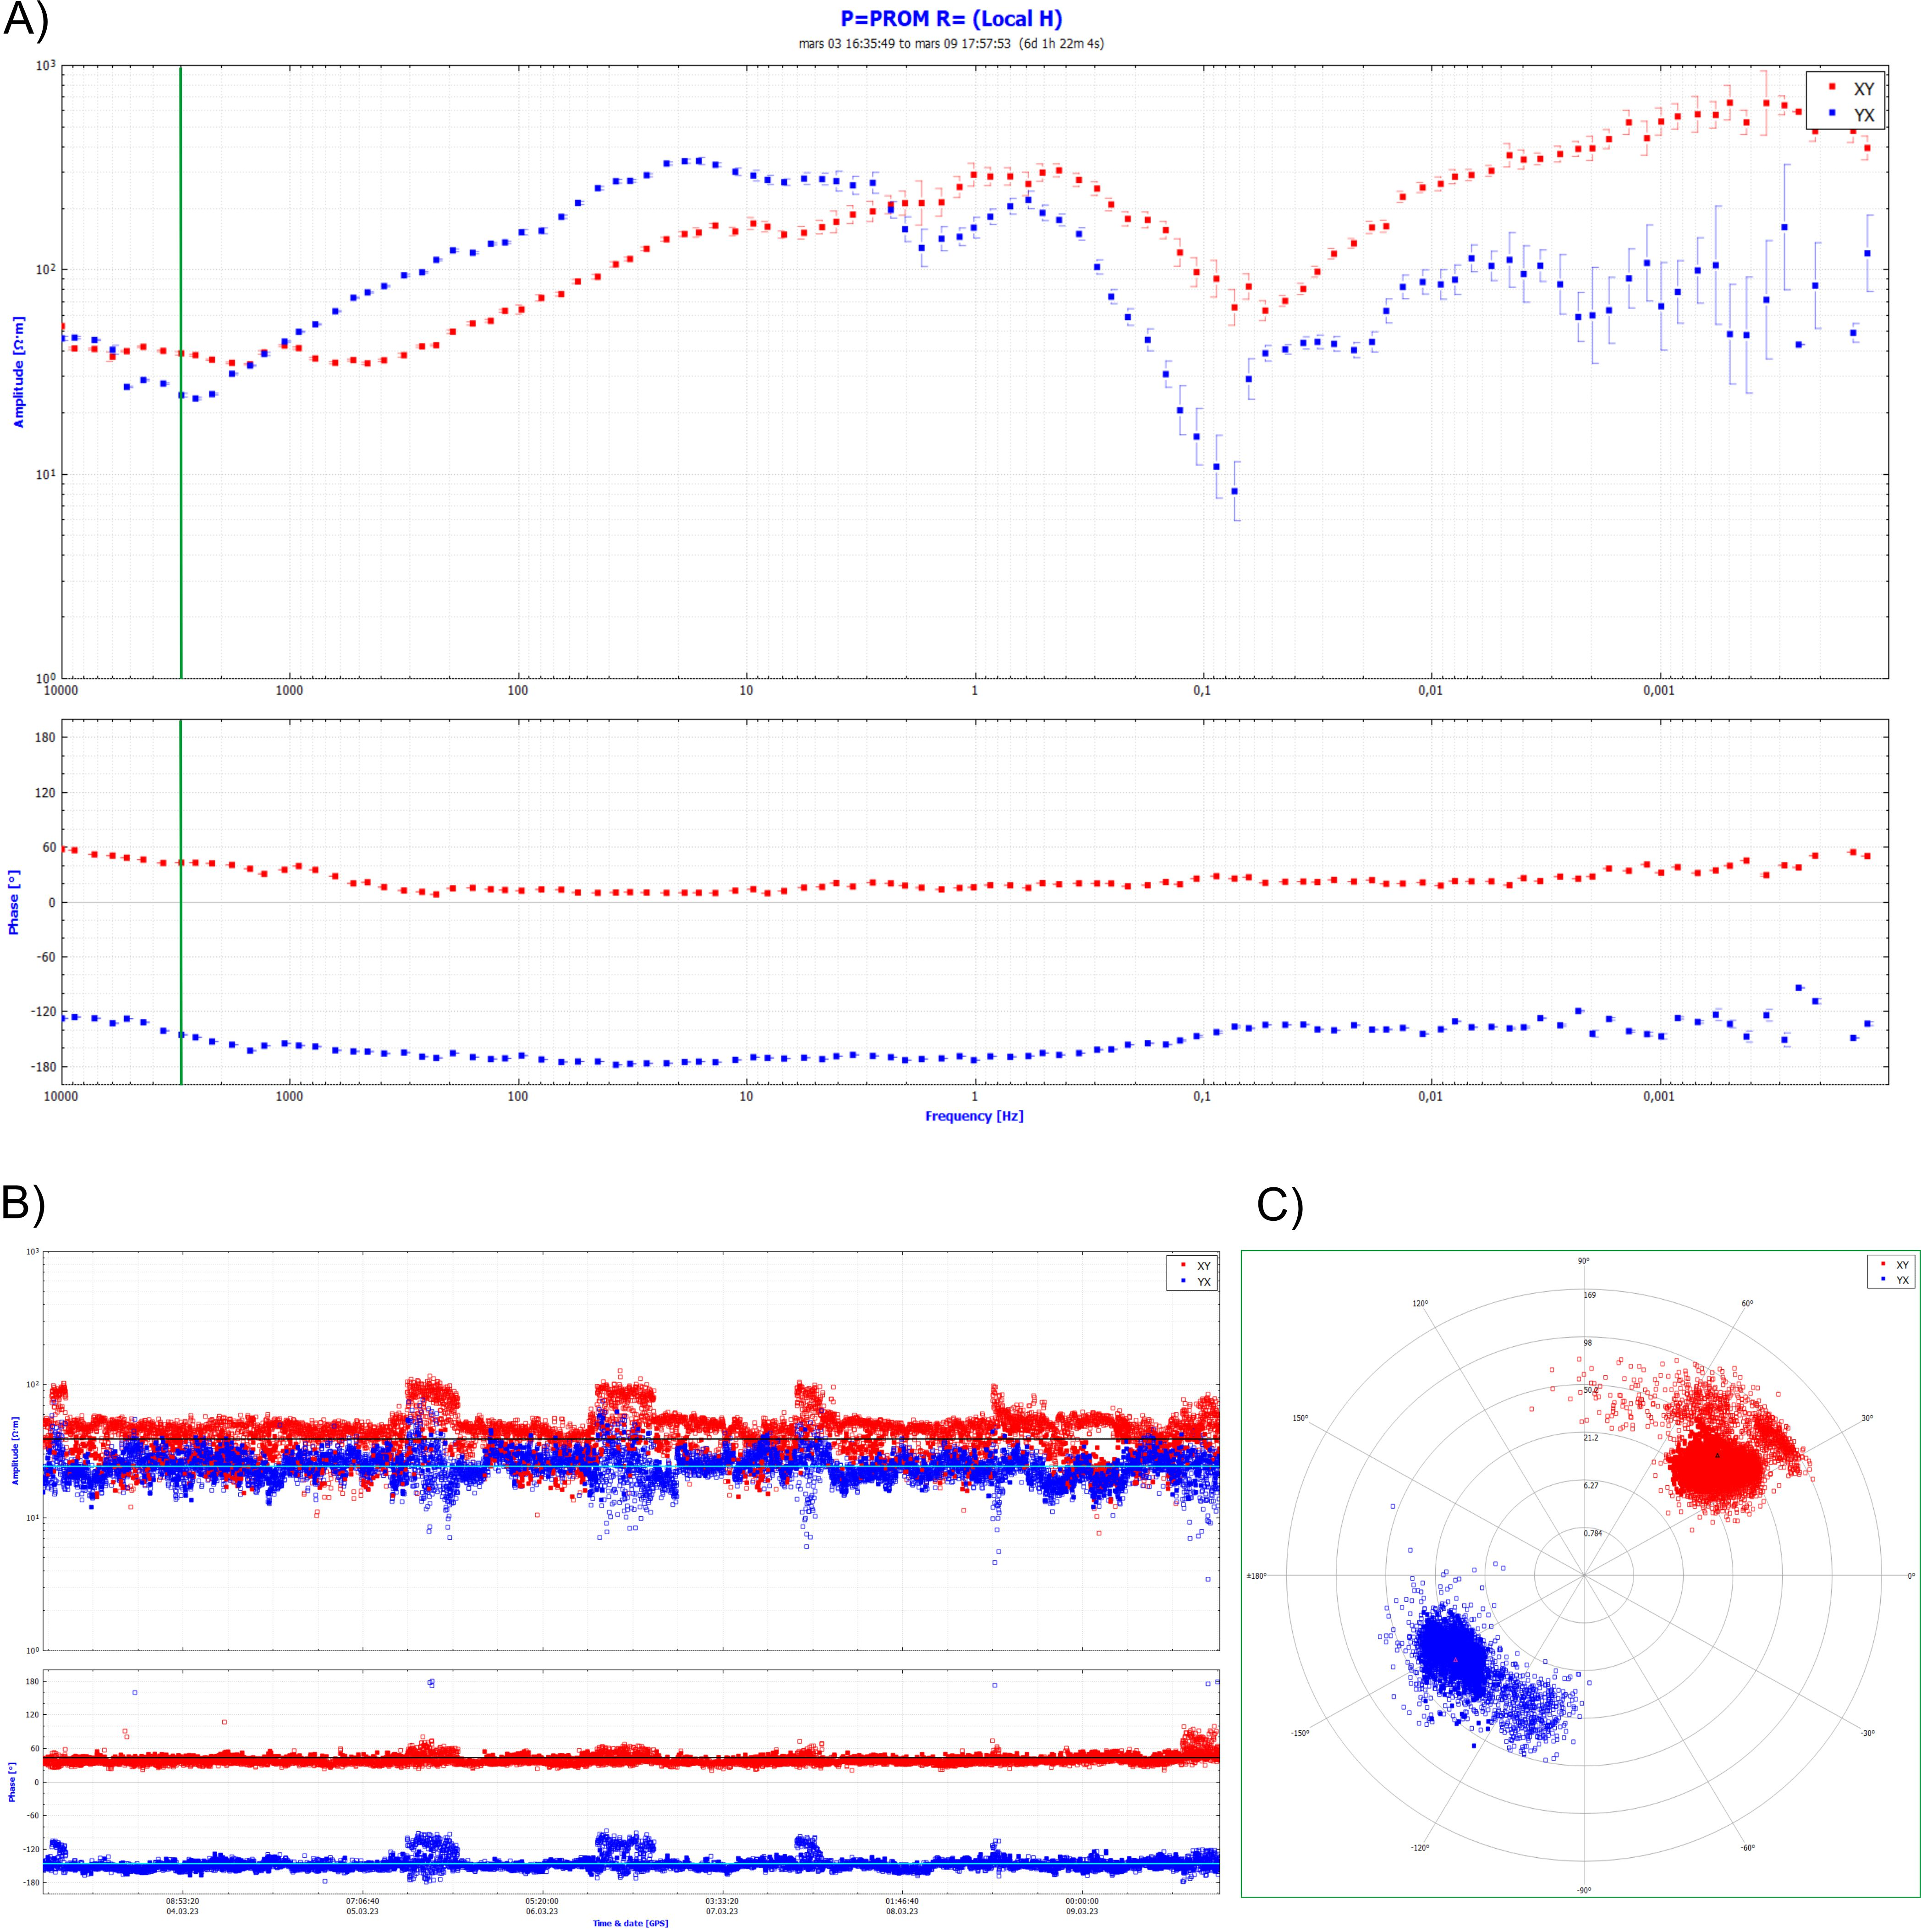
\includegraphics[width = .35\textwidth]{phd-isterre-poster-2023-fig.jpg}
	\end{center}
	\begin{alertblock} {An alert block}
		\begin{itemize}
			\item Number one
			\item Number two
		\end{itemize}
	\end{alertblock}
\end{frame}

\subsection{Frames with columns}
\begin{frame}
    \begin{columns}[c] % c = Vertical centering
        \column{.6\textwidth}
        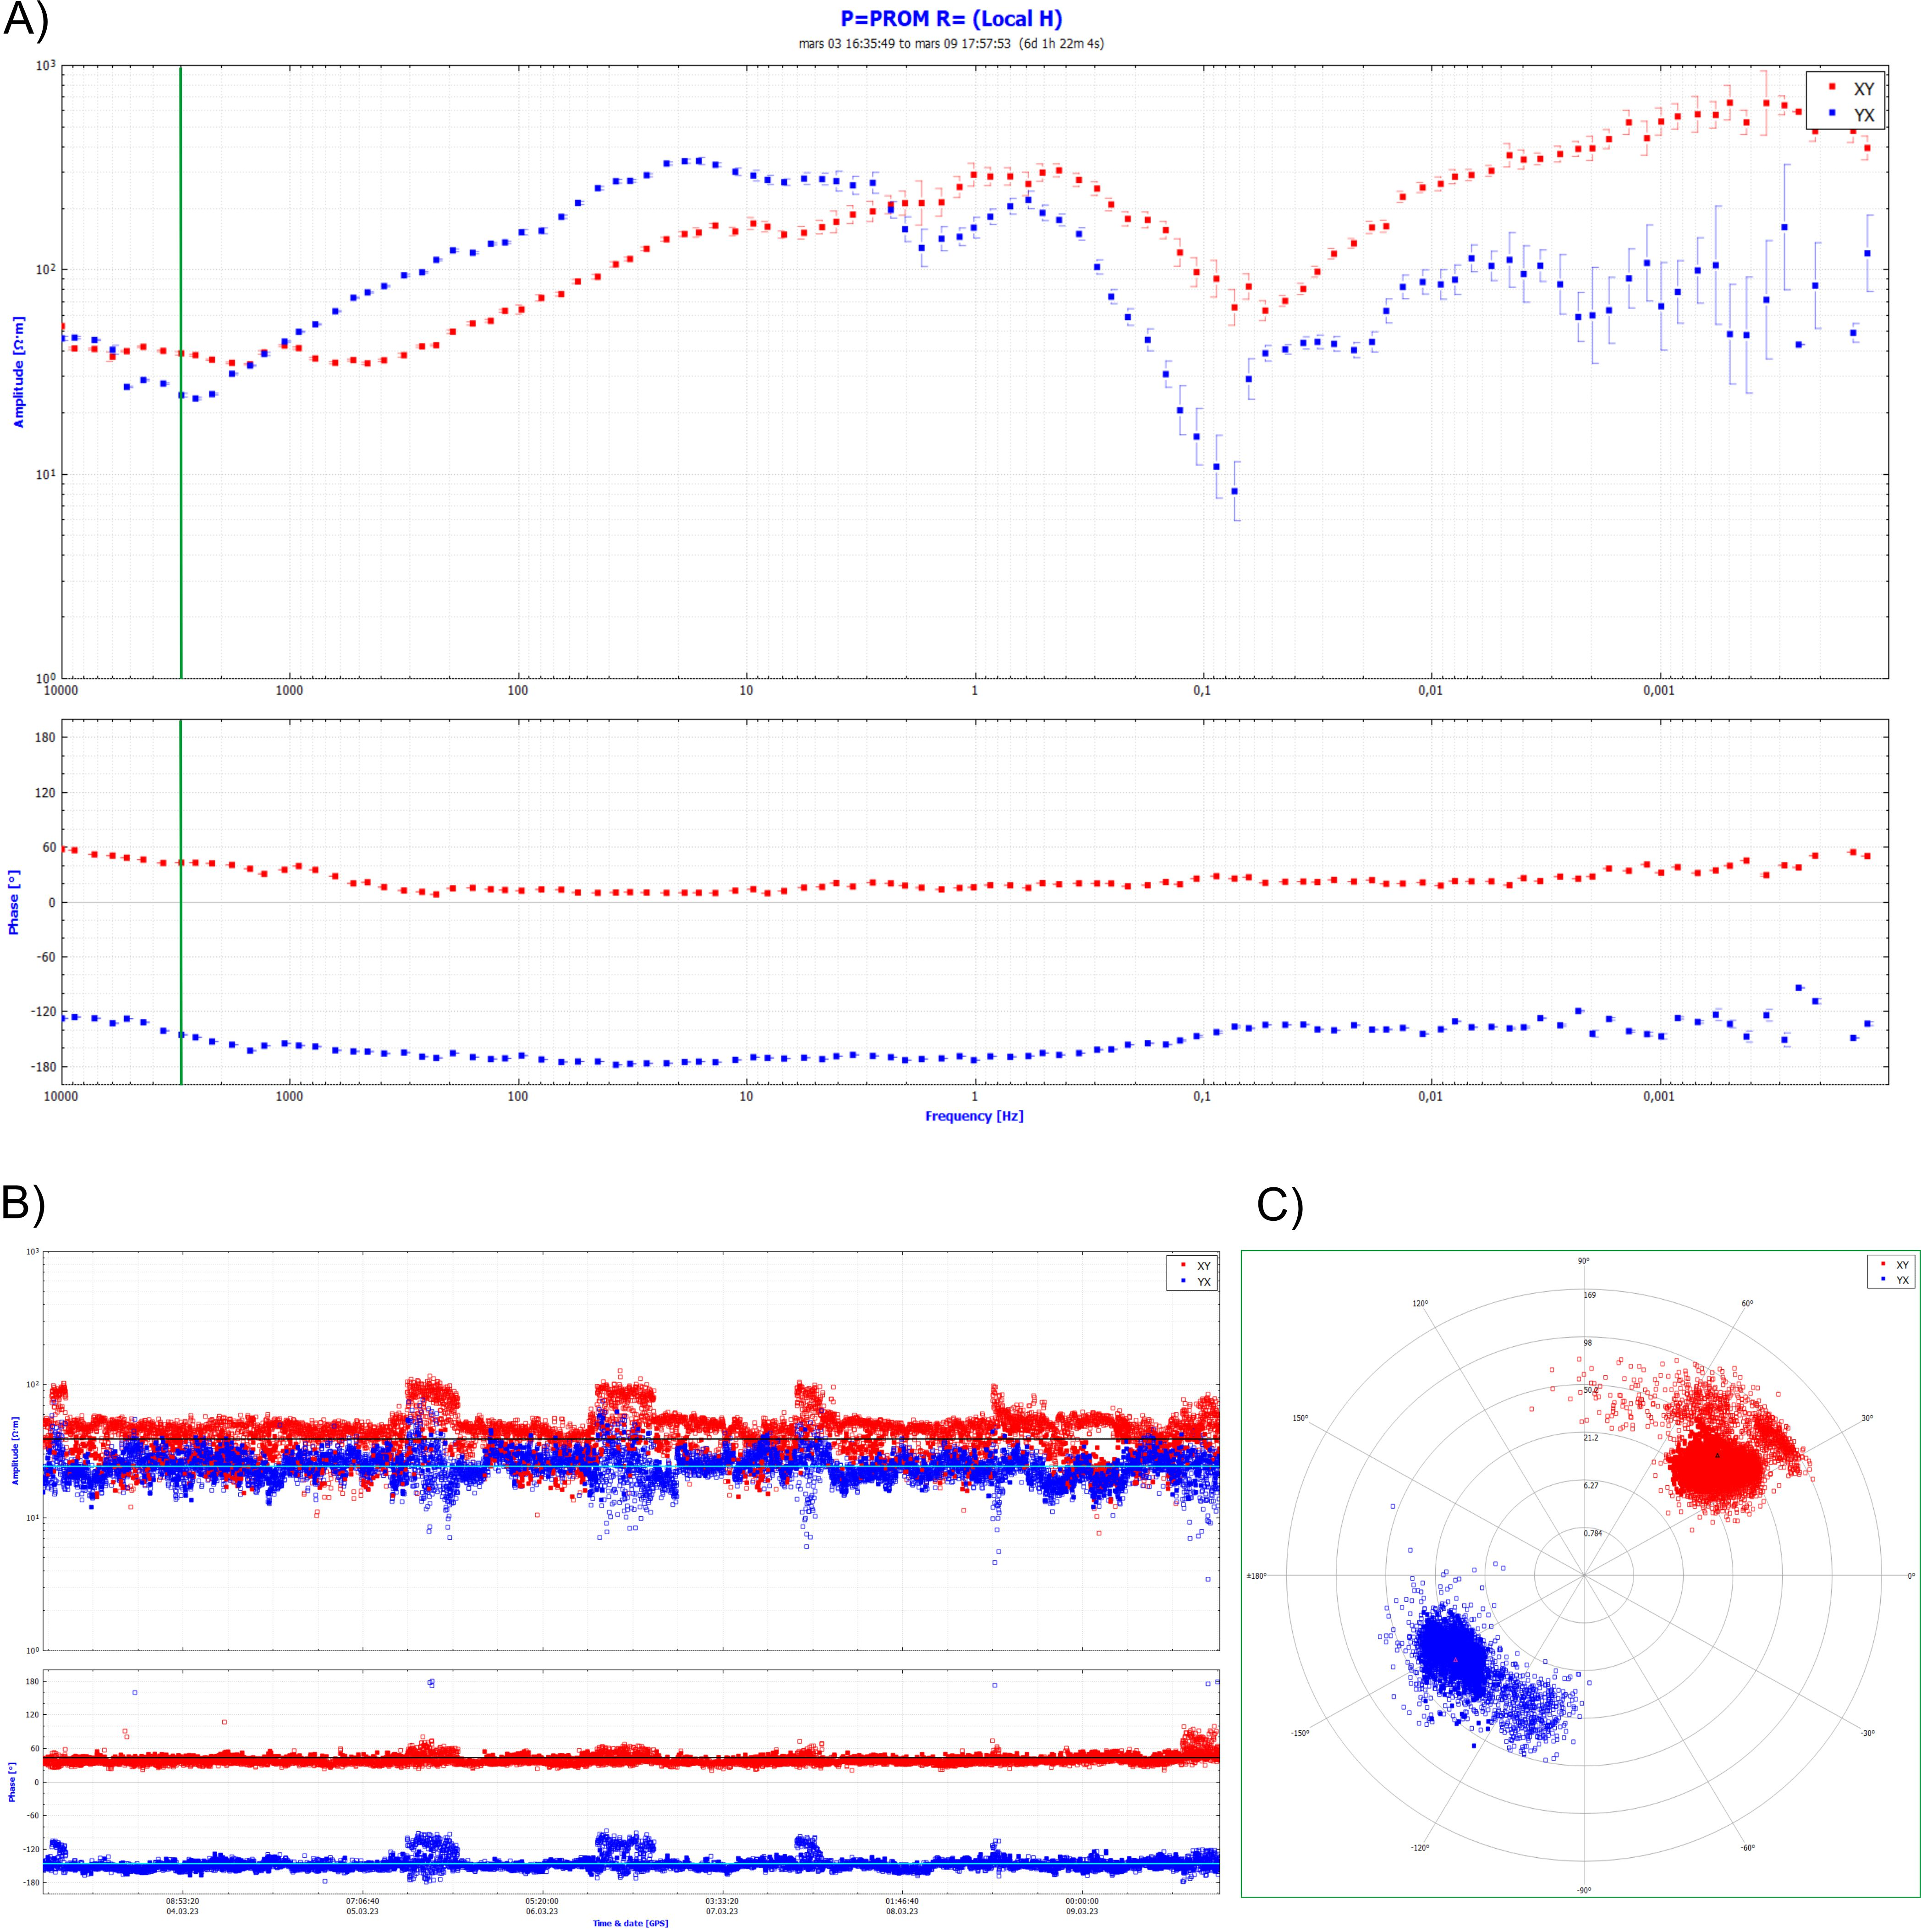
\includegraphics[width = 1.\textwidth]{phd-isterre-poster-2023-fig.jpg}
        \column{.4\textwidth}
        \begin{block}{A standard block}
            \begin{itemize}
                \item Some data.
                \item Some other data.
            \end{itemize}
        \end{block}

        \begin{alertblock}{An alertblock}
            \begin{itemize}
                \item Some data.
                \item Some other data.
            \end{itemize}
        \end{alertblock}
    \end{columns}
\end{frame}


\section{Another more section}
\begin{frame}{Another more section}
	\begin{center}
		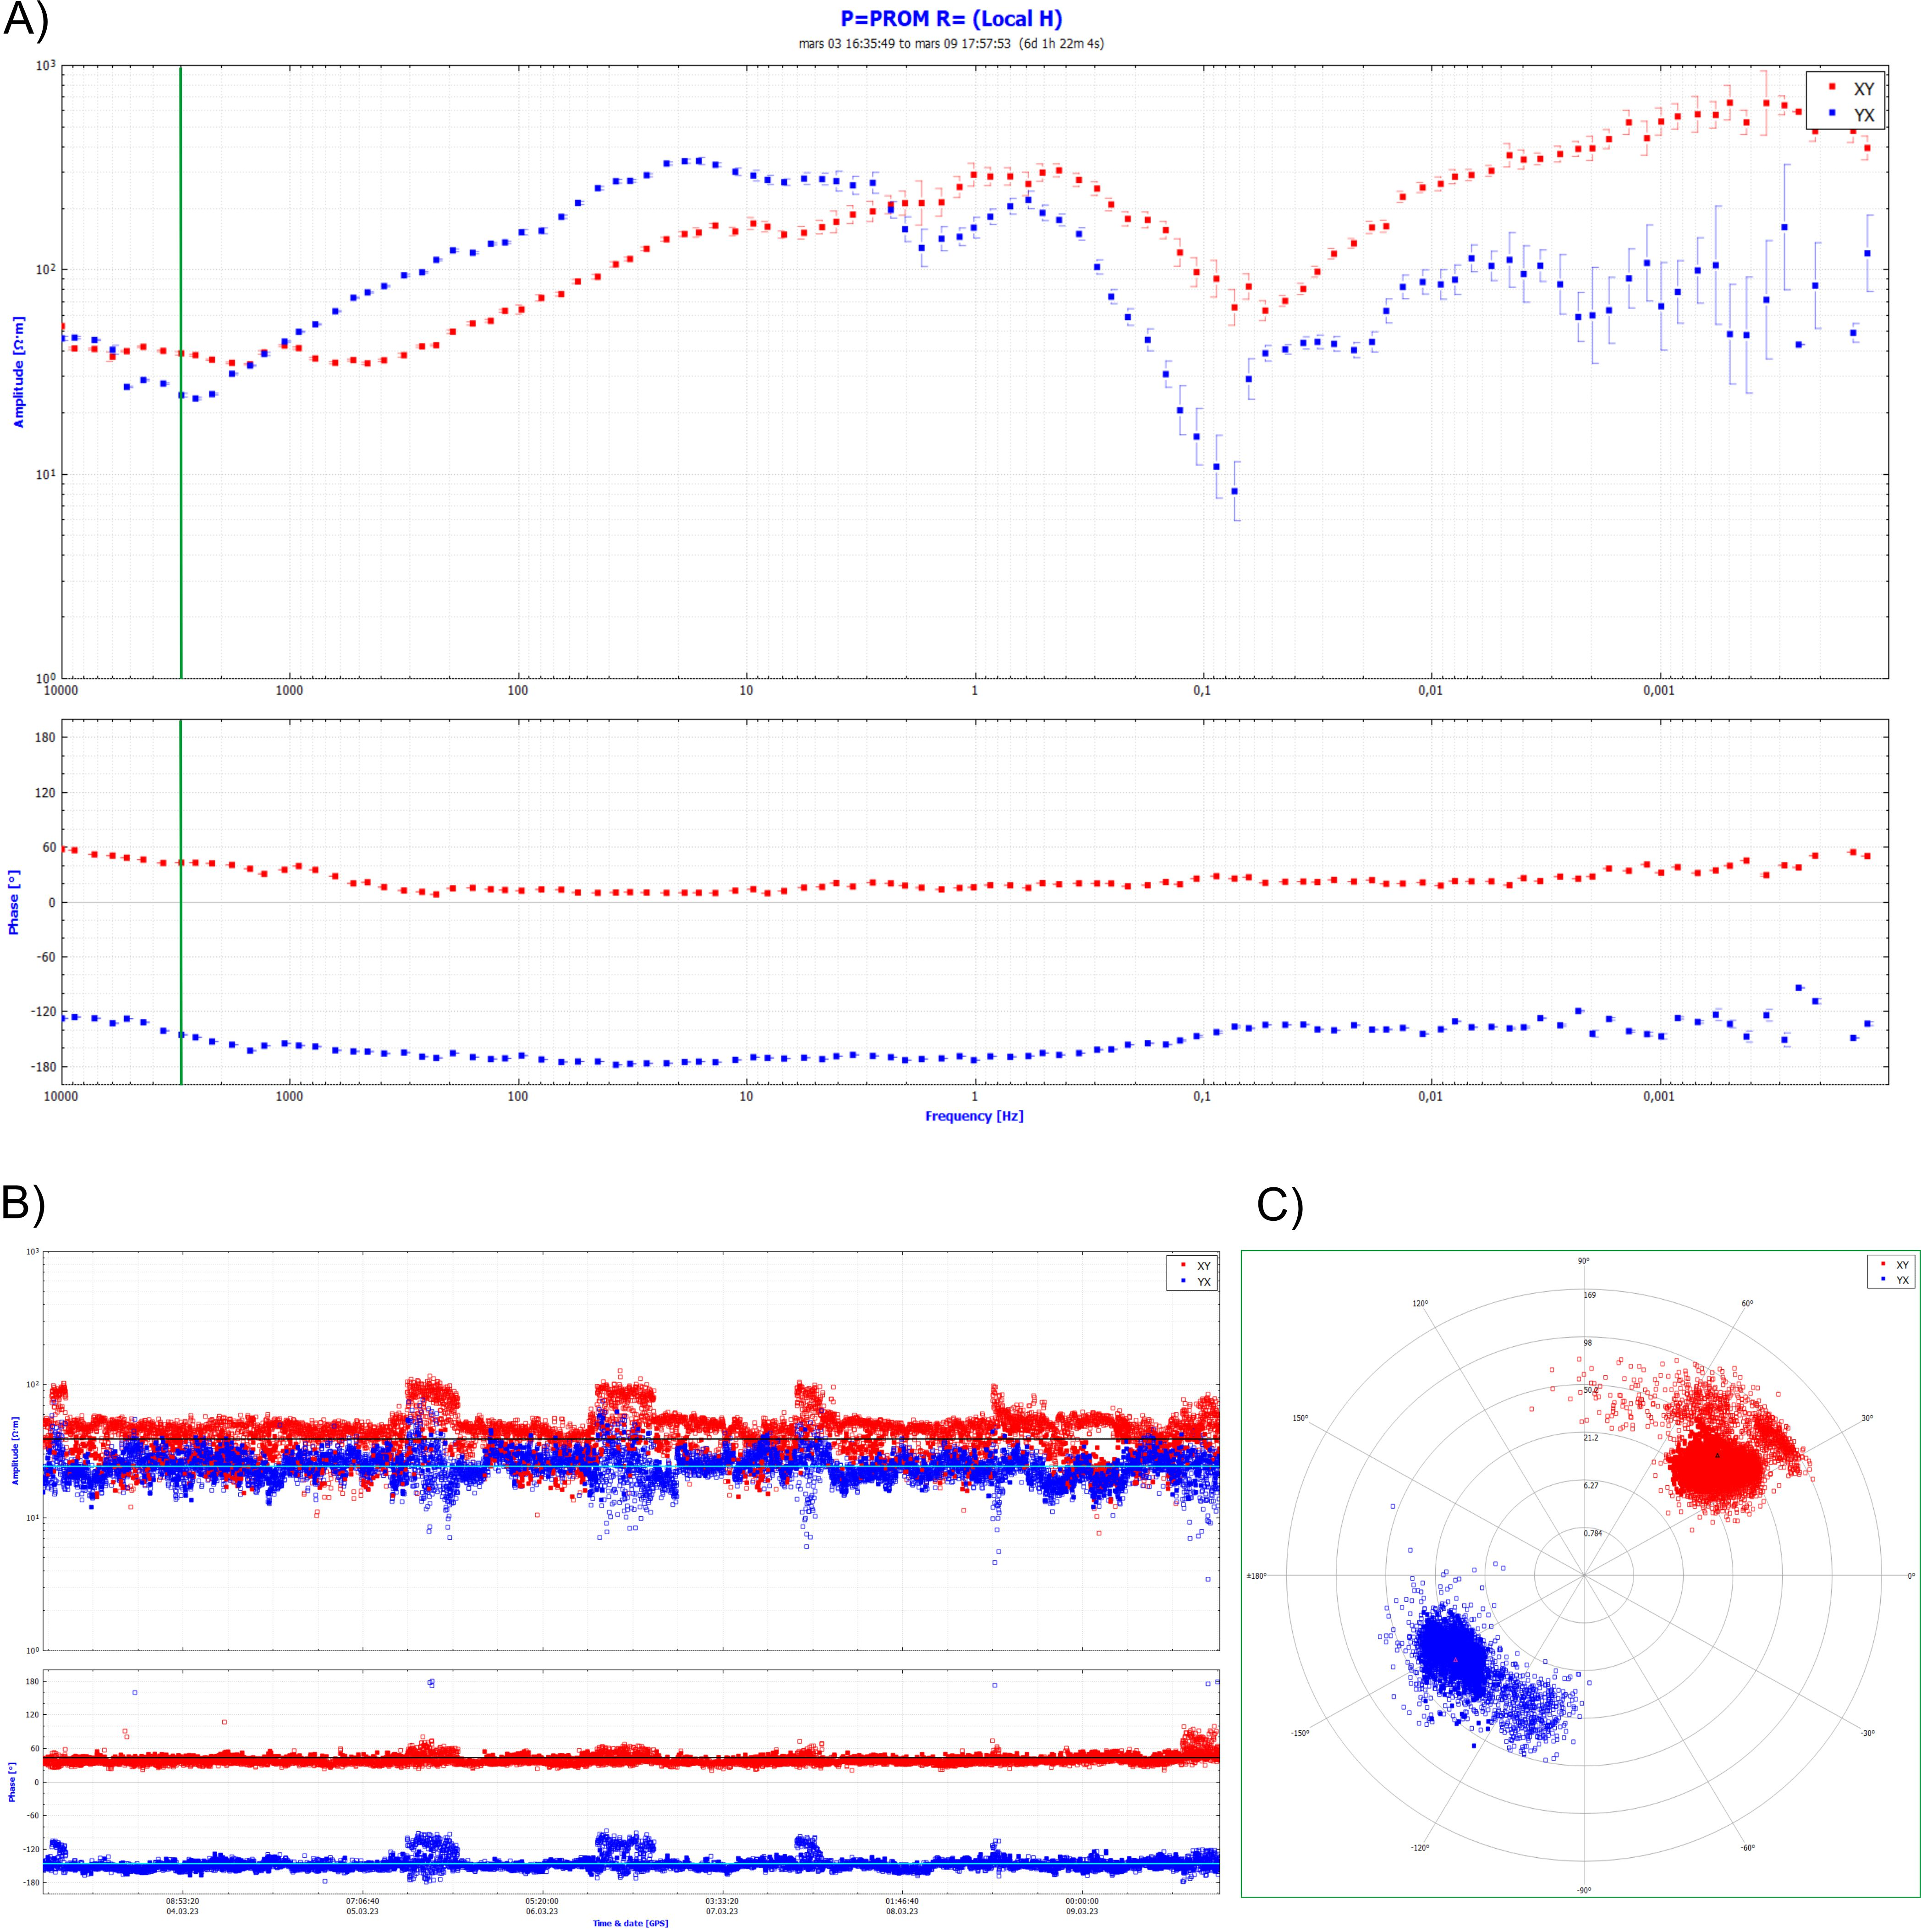
\includegraphics[width = .35\textwidth]{phd-isterre-poster-2023-fig.jpg}
	\end{center}
	\begin{block} {A standard block}
		\begin{itemize}
			\item Number one
			\item Number two
		\end{itemize}
	\end{block}
\end{frame}



\section{Another section}
\begin{frame}{Blocs 1/2}
	\begin{center}
		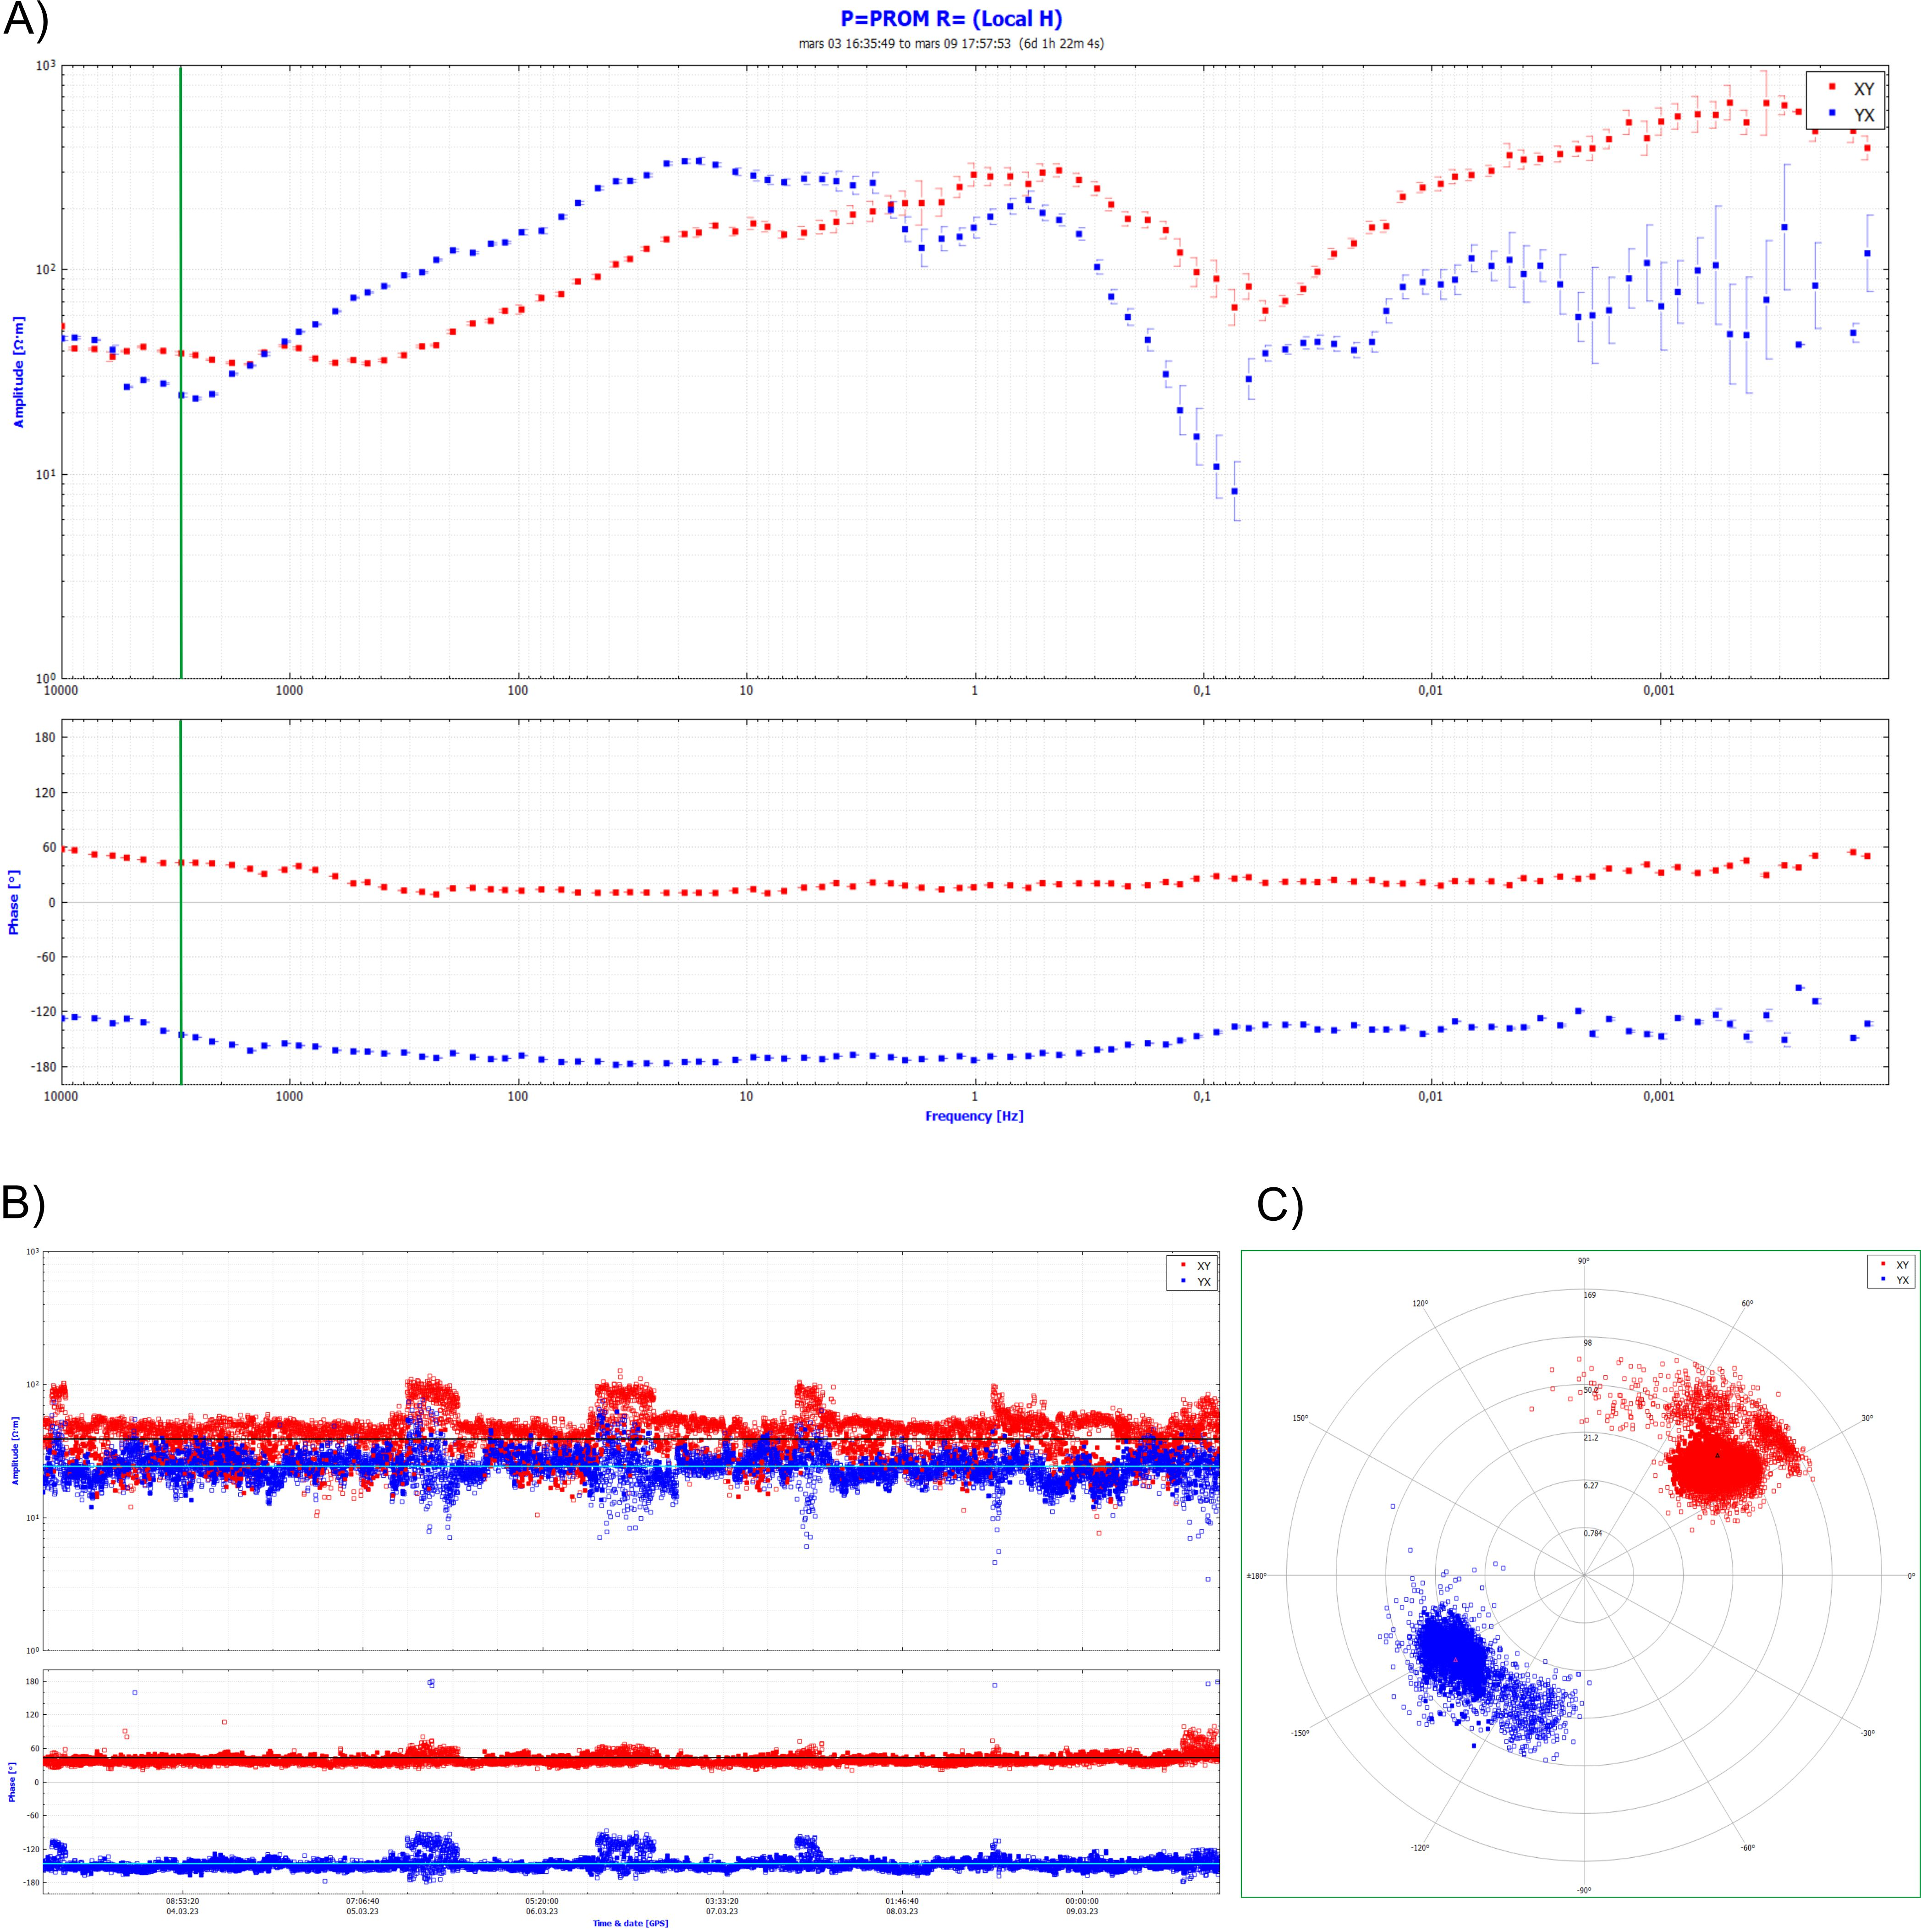
\includegraphics[width = .35\textwidth]{phd-isterre-poster-2023-fig.jpg}
	\end{center}
	\begin{block} {A standard block}
		\begin{itemize}
			\pause
			\item Number one
			\pause
			\item Number two
		\end{itemize}
	\end{block}
\end{frame}




\end{document}
